\documentclass{article}
\usepackage{style-notes}

\newcounter{lecnum} 	% define counter for lecture number
\renewcommand{\thepage}{\thelecnum-\arabic{page}}	% define how page number is displayed (< lecture number > - < page number >)

% define lecture header and page numbers
% NOTE: to call use \lecture{< Lecture # >, < Lecture name >, < Chapter # >, < Chapter name >, < Section #s >}
\newcommand{\lecture}[5]{

    % define headers for first page
    \thispagestyle{empty} % removes page number from page where call is made

    \setcounter{lecnum}{#1}		% set lecture counter to argument specified

    % define header box
    \begin{center}
    \framebox{
      \vbox{\vspace{2mm}
    \hbox to 6.28in {\textbf{MATH 320: Probability} \hfill}
       \vspace{4mm}
       \hbox to 6.28in {{\hfill \Large{Lecture #1: #2} \hfill}}
       \vspace{2mm}
       \hbox to 6.28in {\hfill Chapters #3: #4 \small{(#5)}}
      \vspace{2mm}}
    }
    \end{center}
    \vspace{4mm}
    
    % define headers for subsequent pages
    \fancyhead[LE]{\textit{#2} \hfill \thepage} 		% set left header for even pages
    \fancyhead[RO]{\hfill \thepage}		% set right header for odd pages

}

% define macros (/shortcuts)
\newcommand{\bu}[1]{\textbf{\ul{#1}}}				% shortcut bold and underline text in one command
\newcommand{\blankul}[1]{\rule[-1.5mm]{#1}{0.15mm}}	% shortcut for blank underline, where the only option needed to specify is length (# and units (cm or mm, etc.)))
\newcommand{\dx}[1]{\,\mathrm{d} #1}		% shortcut for dx after integral (variable x)
\newcommand{\integral}[4]{\displaystyle \int_{#1}^{#2} #3 \,\mathrm{d} #4}		% shortcut for large integral with limits and appending formatted dx (variable x)
\newcommand{\ddx}[1]{\frac{\mathrm{d}}{\mathrm{d} #1}\,}		% shortcut for derivative d/dx (variable x)
\newcommand{\e}{\mathrm{e}}		% shortcut for non-italic e in math mode



% 2.2 - 2.3
% NOTES on what didn't cover
% infinite discrete random variable expected value, which uses geometric series sum (Actex 4.2)
% convergence / existence of E(X) (Theory lecture 8 examples and notes, Lazar has just a mini note)
% (Actex) Z-scores and Chebychev's theorem (4.4.4) and Population and Sample Statistics (4.5)
% factorial moments and a way (proof) to write variance in terms of this, specifically E(X(X - 1)) (textbook 2.3, page 60)

% 3.1
% points scattered about (in Theory Lecture 6, maybe others) about the pdf (or pmf) containing the same information as the cdf; I included it here, but definitely there are other mentions of it (with mgfs too)
% --> what did Dr. Kim mean by this: (my comment, theory Lecture 6) Usually, we have the cdf first, and then the pdf. 
% integration by parts proof (lazar 3.1 notes)
% another expected value idea (maybe should be relocated to a different 'notes on what didn't cover' section.... Theorem 2.2.5 from Theory Lecture 8 (expected value of a function rules: e.g. if g(x) > 0 for all x, then E(g(X)) > 0.))

\begin{document}

\lecture{9}{Summary Measures}{2 and 3}{Distributions}{2.2, 2.3, and 3.1}

\bu{Expected value}\bigskip

Data reduction\bigskip
\begin{itemize}
    \item When we try to interpret numerical information that has a wide range of values, we like to reduce our confusion by looking at a single number which summaries the information.
    \item[] Sample of \blankul{1cm} data points $\longrightarrow$ \blankul{1cm} summary measures.    
\end{itemize}\bigskip

Motivating example\bigskip
\begin{itemize}
    \item When the quizzes are returned, students are interested in the quiz average as well as the distribution of grades.
    \item[] Lets say we have the following quiz scores:\hspace{20pt} 6, 7, 8, 9
    \item[] First we are going to calculate the mean like we normally would, then do some rearranging.\vspace{50pt}
    \item[] Written out like this, we can think of \blankul{1cm} as a probability and the numbers as $x$'s, which are particular instances of the random variable $X$. Then we have a probability function.\smallskip
    \begin{center}
    \begin{tabular}{| l || c | c | c | c |}
        \hline
        Quiz score $(x)$ & 6 & 7 & 8 & 9\\
        \hline
        $f(x)$ & 1/4 & 1/4 & 1/4 & 1/4\\
        \hline
    \end{tabular}
    \end{center}\bigskip
    \item[] Now what if we said that a score of 9 is more likely than the other scores. Our new pmf is:
    \begin{center}
    \begin{tabular}{| l || c | c | c | c |}
        \hline
        Quiz score $(x)$ & 6 & 7 & 8 & 9\\
        \hline
        $f(x)$ & 1/6 & 1/6 & 1/6 & 1/2\\
        \hline
    \end{tabular}
    \end{center}\bigskip
    \item[] The new mean going to \blankul{2.5cm}. Let's calculate it:\vspace{40pt}
    \item What we are actually calculating here is called the \blankul{3cm}, which we can think of as a \blankul{4cm} of the \blankul{1cm} where the \blankul{4cm} are the weights.
    \item[] This is how we get mean (aka expected value) of a random variable from its pmf, which is usually what we are given.
\end{itemize}\bigskip

Defining expected value\bigskip
\begin{itemize}
    \item Definitions
    \item[] Let $X$ be a discrete random variable. The \textbf{expected value} of $X$ is defined by\smallskip
    \[E(X) = \hspace{50pt}\]
    \item[] Let $X$ be a continuous random variable. The \textbf{expected value} of $X$ is defined by
    \[E(X) = \hspace{50pt}\]
    \item[] The expected value of the random variable $X$ is often denoted by the Greek letter $\mu$.
    \[E(X) = \hspace{50pt}\]
    \item Examples
    \begin{enumerate}
        \item Pmf for the random variable $X$, the number of health insurance claims filed by a policyholder in a year, is given in the table below.\smallskip
        \begin{center}
            \begin{tabular}{| l || c | c | c | c | c |}
                \hline
                Number of claims $(x)$ & 0 & 1 & 2 & 3\\
                \hline
                $f(x)$ & 0.28 & 0.43 & 0.20 & 0.09\\
                \hline
            \end{tabular}
        \end{center}\bigskip
        \item[] Find the expected number of claims.\vspace{70pt}
        \item Let $X$ be the loss severity random variable for the warranty policy with density:
        \[
        f(x) =
        \left\{
            \begin{array}{ll}
            0.02 - 0.0002x & 0 \le x \le 100\\
            0 & \text{otherwise}
        \end{array}
        \right.
        \]
        \item[] Find the expected loss.\vspace{70pt}
        \item Expected value of a piecewise density function example: Let $X$ have the following pdf:\smallskip
        \[
        f_X(x) =
            \left\{
            \begin{array}{ll}
                560x & 0 \le x \le 0.05\\
                -15x + 3.75 & 0.05 < x \le 0.25\\
                0 & \text{otherwise}\\
            \end{array}
            \right.
        \]
        \item[] Find the expected value.
        \begin{itemize}
            \item \textit{STRATEGY:} Integrate in pieces.
        \end{itemize}\vspace{90pt}
        \item Smith is offered the following gamble: he is to choose a coin at random from a large collection of coins and toss it randomly.
        \begin{itemize}
            \item 3/4 of the coins in the collection are loaded toward head ($LH$) and 1/4 are loaded towards a tail ($LT$).
            \item If a coin is loaded towards a head, then when the coin is tossed randomly, there is a 3/4 probability that a head will turn up and a 1/4 probability that a tail will turn up. Similarly, if the coin is loaded towards tails, then there is a 3/4 chance of tossing a tail on any given toss.
            \item If Smith tosses a head, he loses \$100 and if he tosses a tail, he wins \$200.
            \item Smith is allowed to obtain ``sample information'' about the gamble. When he chooses the coin at random, he is allowed to toss it once before deciding to accept the gamble with that same coin.
        \end{itemize}
        \item[] Suppose Smith tosses a head on the sample toss. Find Smith's expected gain/loss on the gamble if it is accepted.\vspace{200pt}
    \end{enumerate}
\end{itemize}\bigskip


\bu{Expected value of a function of a random variable}\bigskip

Motivating example\bigskip\
\begin{itemize}
    \item Suppose $X$ is a random variable, but we are actually interested in a function of the random variable $g(X)$ (which is another random variable). 
    \item[] One common application of this is when $g(X) = aX + b$.\bigskip
    \item Now suppose the table from the previous Example 1 is for a type of policy which guarantees a fixed payment of \$100 dollars for each claim.
    \item[] Then the amount paid to a policy holder in a year is just \$100 multiplied by the number of claims. The total claim amount is a new random variable \blankul{2cm}.
    \item[] We now have two random variables, $X$ and $Y$, and each has their own pmf.\bigskip
    \begin{center}
        \begin{tabular}{| l || c | c | c | c |}
            \hline
            Number of claims $(x)$ & 0 & 1 & 2 & 3\\
            \specialrule{.1em}{.05em}{.05em}
            Total claim amount $(y)$ & \hspace{30pt} & \hspace{30pt} & \hspace{30pt} & \hspace{30pt} \\
            \hline
            $f(y)$ & \hspace{30pt} & \hspace{30pt} & \hspace{30pt} & \hspace{30pt} \\
            \hline
        \end{tabular}
    \end{center}\bigskip
    \begin{enumerate}[(a)]
        \item Find the expected total claim amount.\vspace{140pt}
    \end{enumerate}\bigskip
\end{itemize}\bigskip
     
 Theorems\bigskip
 \begin{itemize}
    \item Theorem: For any constant $a$ and random variable $X$,
    \[E(aX) = \]
    \item[] We can derive this!\vspace{140pt}
    \item Transformation mapping
    \begin{itemize}
        \item If $Y = g(X)$ is a one-to-one function, then the inverse of $g(X)$ exists. So we can go ``backwards'' in our mapping.\vspace{140pt}
    \end{itemize}
    \item We can also extend this rule for adding a constant. Continuing example:
    \begin{enumerate}[(a)]\setcounter{enumi}{1}
        \item Lets say the insurance company has a yearly fixed cost of \$20 per policyholder for administering the insurance policy. So the total cost in a year for a policy is the sum of the claim payments and the administrative cost.
        \item[] Write our new random variable for the total cost and find the expected cost per policy per year.\bigskip\\
        \begin{tabular}{| c | c | c | c |}
            \hline
            $x$ & $f(x)$ & $z = \hspace{50pt}$ & $f(z)$ \\
            \specialrule{.1em}{.05em}{.05em}
            0 & 0.28  & & \\
            \hline
            1 & 0.43  & & \\
            \hline
            2 & 0.20 & & \\
            \hline
            3 & 0.09  & & \\
            \hline
        \end{tabular}\vspace{100pt}
    \end{enumerate}
    \item Theorem: For any constants $a$ and $b$ and random variable $X$,
    \[E(aX + b) = \]
    \item[] Discrete derivation:\vspace{140pt}
    \item[] Continuous derivation:\vspace{80pt}
    \item Simple example: Continuing previous example 2. Suppose that due to inflation the losses on the warranty policy are expected to increase by 5\% and have an additional fixed cost of \$30 for the following year. Find the expected value for the following year.\vspace{30pt}
    \item Theorem: For some constant random variable $X = a$,
    \[E(X) = E(a) = a\]
    \item[] (Discrete) Derivation:\vspace{70pt}    
\end{itemize}\bigskip

Generalizing expected value of a function of a random variable\bigskip
\begin{itemize}
    \item Now suppose we are working with functions that are more complex than $Y = g(X) = aX + b$, specifically functions that are not one-to-one function. Let's see how to find the expected value when this is the case.
    \item Example: Let $X$ be a discrete random variable with the pmf given below. Find the expected value of $Y = g(X) = X^2$.\bigskip\\
    \begin{tabular}{| l || c | c | c | c |}
        \hline
        $x$ \hspace{20pt} & \hspace{10pt} -1 \hspace{10pt} & \hspace{10pt} 0 \hspace{10pt} & \hspace{10pt} 1 \hspace{10pt} \\
        \hline
        $f(x)$ & 0.2 & 0.6 & 0.20\\
        \hline
    \end{tabular}\vspace{100pt}
    \item[] More complex because $g(X)$ is \blankul{5cm} function.
    \item This example illustrates two major points.
    \begin{enumerate}
        \item The distribution table for $X$ can be converted into a preliminary table for $g(X)$ with entries for $g(x)$ and $f(x)$, but some regrouping may be necessary to get the actual distribution table for $Y = g(X)$.
        \item Even though the tables are not the same, they lead to the same results for the expected value of $Y = g(X)$.
    \end{enumerate}\bigskip
    \item Theorem:
    \item[] Let $X$ be a discrete random variable. The \textbf{expected value} of $Y = g(X)$ is given by\smallskip
    \[E(Y) = \hspace{200pt}\]\vspace{30pt}
    \item[] Let $X$ be a continuous random variable. The \textbf{expected value} of $Y = g(X)$ is given by\smallskip
    \[E(Y) = \hspace{200pt}\]\vspace{40pt}
    \item Examples:
    \begin{enumerate}
        \item Let the random variable $X$ have the pmf $f(x) = \frac{x}{10} \quad \text{for } x = 1, 2, 3, 4$.
        \item[] Find $E(X^2)$ and $E[X(5-X)]$.\vspace{80pt}
        \item Let $f(x) = 3x^{-4} \quad \text{for } x > 1$. Find $E(2X^2)$.\vspace{100pt}
    \end{enumerate}
\end{itemize}

\bu{Variance and standard deviation}\bigskip

Measures of spread\bigskip
\begin{itemize}
    \item The mean of a random variable gives a nice single summary number to measure \blankul{2.5cm} tendency. However two different random variables can have the same mean and still be quite different.\vspace{40pt}
\end{itemize}\bigskip

Motivating example\bigskip
\begin{itemize}
    \item Below is the pmfs of quiz scores for two different classes.
    \begin{enumerate}[(a)]
        \item Find the mean of each.\bigskip\\
        Class 1: RV $X$ \hspace{10pt}
        \begin{tabular}{| l || c | c | c |}
            \hline
            Score $(x)$ & 7 & 8 & 9 \\
            \hline
            $f(x)$ & 0.2 & 0.6 & 0.2 \\
            \hline
        \end{tabular}\bigskip\\
        Class 2: RV $Y$ \hspace{10pt}
        \begin{tabular}{| l || c | c | c |}
            \hline
            Score $(y)$ & 6 & 8 & 10 \\
            \hline
            $f(y)$ & 0.2 & 0.6 & 0.2 \\
            \hline
        \end{tabular}\vspace{80pt}
        \item[] Means are the \blankul{2cm}, but obviously the two random variables are quite different. There is much more variation or dispersion in $Y$ than $X$. The question is, how to measure that variation?
        \item We could look at the distance between each individual value of $x$ or $y$ from the mean of its distribution.\vspace{30pt}
        \item[] This is always true for any random variable.
        \item However, if we look at the square of the distance between the mean, this problem does not occur. Now find the expected values of each of these new pmfs.\bigskip\\
        RV = $(X - \mu_X)^2$ \hspace{10pt}
\begin{tabular}{| l || c | c | c |}
            \hline
             $(x - 8)^2$ & $(7 - 8)^2 = 1$ & $(8 - 8)^2 = 0$ & $(9 - 8)^2 = 1$ \\
            \hline
            $f(x)$ & 0.2 & 0.6 & 0.2 \\
            \hline
        \end{tabular}\bigskip\\
        RV = $(Y - \mu_Y)^2$ \hspace{10pt}
        \begin{tabular}{| l || c | c | c |}
            \hline
             $(y - 8)^2$ & $(6 - 8)^2 = 4$ & $(8 - 8)^2 = 0$ & $(10 - 8)^2 = 4$ \\
            \hline
            $f(y)$ & 0.2 & 0.6 & 0.2 \\
            \hline
        \end{tabular}\vspace{50pt}
    \end{enumerate}
    \item This is the single measure of variation that is most widely used in probability theory.
\end{itemize}\bigskip

Defining variance and standard deviation\bigskip
\begin{itemize}
    \item Definition: The \textbf{variance} of a random variable $X$ is defined to be
    \[V(X) = \hspace{10pt}\]
    \item Definition: The \textbf{standard deviation} of a random variable is the square root of its variance. It is denoted by the greek letter $\sigma$.
    \[\sigma = \hspace{10pt}\]
    \item Notes
    \begin{itemize}
        \item The variance is also written as \blankul{1cm}.
        \item $SD(X)$ is in the same units as $X$ and $V(X)$ is in \blankul{2cm}.
        \item Variance is just a special expected value with $g(X) = (X -\mu)^2$.\bigskip
    \end{itemize}\bigskip
    \item Definitions:
    \item[] \hspace{20pt} \ul{Discrete} \hspace{100pt} \ul{Continuous}\vspace{40pt}
    \item Examples:
    \begin{enumerate}
        \item Let $X$ be the random variable with $f(x) = (3/8)x^2 \quad \text{for } 0 < x < 2$. Find $\sigma^2_X$.\vspace{200pt}
        \item Let $\displaystyle f(x) = \frac{3x + 4}{22} \quad \text{for } x = -1, 0, 1, 2$.
        \item[] Find the mean, variance and standard deviation of $X$.\vspace{150pt}
    \end{enumerate}
\end{itemize}\bigskip

Expectation as a linear operator\bigskip
\begin{itemize}
    \item Now lets say we want to find the expected value of $g(X) = (X - 3)^2 = X^2 -6X + 9$.
    \item[] This is a more complicated function of $X$ because it has multiple $X$'s. To find the expected value of $g(X)$ in this case, we can do what intuitively makes sense.\vspace{80pt}
    \item Theorem: The reason this works is because of the following property of expectation:
    \[E\bigg[\sum_{i = 1}^k c_i g_i(X)\bigg] = \sum_{i = 1}^k c_i E[g_i(X)]\]
    \item[] In fancy words, the expected value of a linear combination equals a linear combination of expected values.
    \item Because of the property, expectation is often called a \textbf{linear (or distributive) \\operator}.
    \item[] Integration and derivation are linear operators as well:
    \item[] $\integral{}{}{[g(x) + f(x)]}{x} = $
    \item[] $\ddx{x} \big[g(x) + f(x)] = $
\end{itemize}\newpage

Another way to calculate variance\bigskip
\begin{itemize}
    \item Using the property we just showed for expectation, we can arrive at another way to calculate the variance of a random variable.\vspace{140pt}
    \item Theorem: Another way to calculate variance:
    \[V(X) = \hspace{200pt}\]\vspace{30pt}
    \item Examples:
    \begin{enumerate}
        \item Below is a pmf table for $X$.\bigskip\\
        \begin{tabular}{| l || c | c | c | c | c |}
            \hline
            $x$ & 0 & 1 & 2 & 3\\
            \hline
            $f(x)$ & 0.5 & 0.3 & 0.06 & 0.14\\
            \hline
        \end{tabular}\bigskip
        \item[] Find $V(X)$ using the new formula.\vspace{70pt}
        \item Find the variance of the warranty loss random variable using the alternate formula.    
        \[
        f(x) =
            \left\{
            \begin{array}{ll}
                 0.02 - 0.0002x & 0 \le x \le 100\\
                 0 & \text{otherwise}
            \end{array}
            \right.
        \]\vspace{80pt}
        \item[] Calculating the variance from the definition would require evaluation of the integral:
        \[V(X) = \integral{0}{100}{\Big(x - \frac{100}{3}\Big)^2 (0.02 - 0.0002x)}{x}\]
        \item[] This would be straightforward, but time consuming relative the the other way if done by hand. Of course with computing, calculation time is not an issue.
    \end{enumerate}
    \item Important practical note: The calculation of variance can be done more easily by hand using this alternate form rather than the definition.
    \item[] But using the definition is more efficient for computers when large values of $X$ are present (problems with overflow due to the magnitude of $X^2$).
\end{itemize}\bigskip

Technology session\bigskip
\begin{itemize}
    \item Using TI-84 (and TI-30XS MultiView) to calculate $E(X)$ and $SD(X)$.
\end{itemize}\bigskip

\begin{figure}[H]
    \center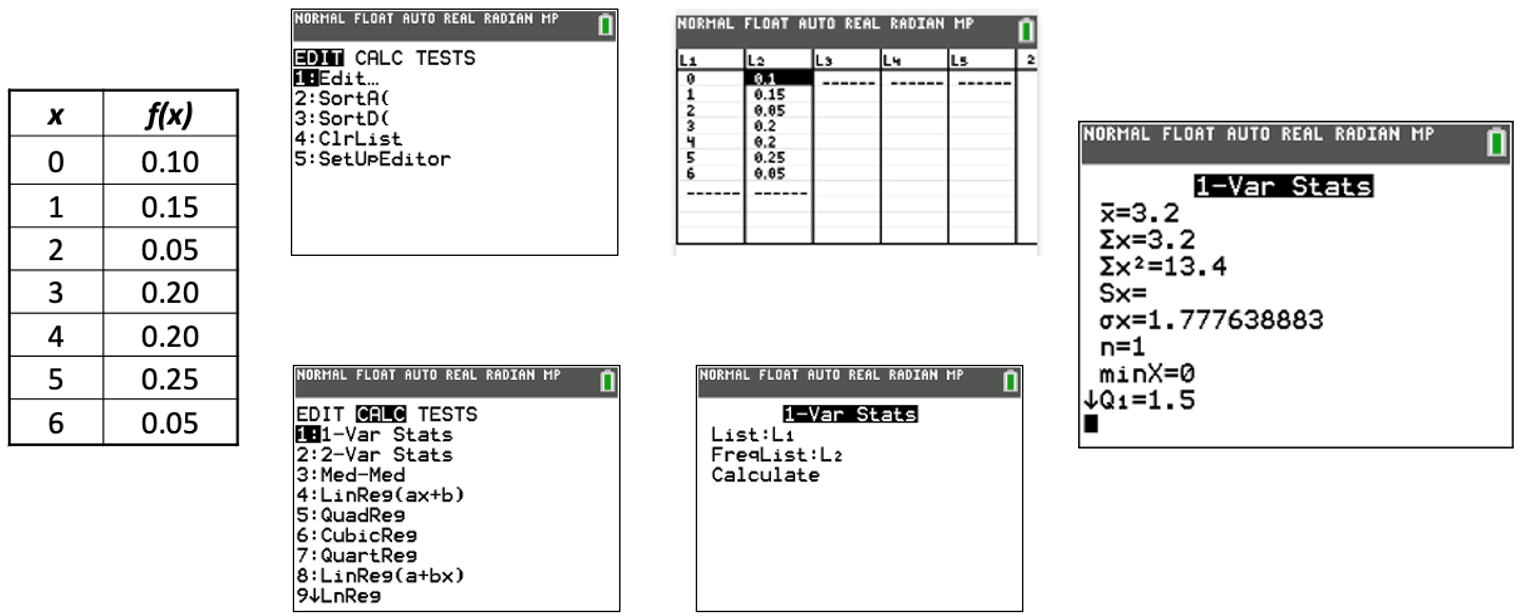
\includegraphics[scale=0.6]{test-2/1-var-stats}
\end{figure}\newpage

\bu{Variance and standard deviation of a function of a random variable}\bigskip

Variance and standard deviation of $Y = aX + b$\bigskip
\begin{itemize}
    \item Previously, we saw how multiplying by a coefficient $a$ and adding a constant $b$ affected the expected value of our new random variable $Y = aX + b$. Now let's study the affect they have on the variance and standard deviation.
    \item First we will look at only the affect of the coefficient.\vspace{80pt}
    \item[] Derivation of $V(aX)$:\vspace{100pt}
    \item Theorem: For any constant $a$ and random variable $X$,\hspace{30pt} (alternate notation)
    \[V(aX) = \hspace{130pt} \sigma^2_{aX} =\]
    \item[] The standard deviation of $aX$ can now be obtained by taking the square root.
    \[SD(aX) = \hspace{130pt} \sigma_{aX} = \]\smallskip
    \item Intuitively, here's why the $a$ is squared for $V(aX)$:\vspace{60pt}
    \item Example: Using the previous quiz scores from class 1, lets investigate two different types of curves the instructor could use and their impact on the expected value and variance.
    \begin{itemize}
        \item Curve 1: Each individual score is raised by 25\%.\vspace{80pt}
        \item Curve 2: Every score gets and additional 2 points.\bigskip\bigskip\\
    \end{itemize}
    \begin{tabular}{| l || c | c | c |}
        \hline
        Original score $(x)$ & 7 & 8 & 9 \\
        \specialrule{.1em}{.05em}{.05em}
        Curved score $(c_2)$ & & & \\
        \hline
        $f(c_2)$ & 0.2 & 0.6 & 0.2 \\
        \hline
    \end{tabular}\vspace{180pt}
    \item This example shows the intuitive idea that if all values are shifted by exactly $b$ units, the mean changes but the dispersion around the new mean is exactly the same as before.\bigskip
    \item Theorem: For any constants $a$ and $b$ and random variable $X$,
    \[V(aX + b) = \]
    \item Example:  Let's say your Test 1 grades $X$ had the pmf given below (grades were out of 100 points).
    \item[] The test corrections gave you 1/2 of the missed points back. Find the expected value and standard deviation of the grades after test corrections. Compare this to the original expected value and standard deviation.
    \begin{enumerate}[(a)]
        \item Define a new random variable $Y =$ grade after test corrections.\bigskip\\
        \begin{tabular}{| c | c |}
            \hline
            Grade $(x)$ & $f(x)$ \\
            \specialrule{.1em}{.05em}{.05em}
            60 & 0.02 \\
            \hline
            65 & 0.04\\
            \hline
            70 & 0.17 \\
            \hline
            75 & 0.23 \\
            \hline
            80 & 0.21 \\
            \hline
            85 & 0.15 \\
            \hline
            90 & 0.12 \\
            \hline
            95 & 0.05 \\
            \hline
            100 & 0.01 \\
            \hline
        \end{tabular}\bigskip
        \item Calculate $E(Y)$ and $SD(Y)$.
        \item[] \ul{Short way} $\rightarrow$ $E(Y)$ \& $V(Y)$ indirectly \hspace{10pt} \ul{Long way} $\rightarrow$ $E(Y)$ \& $SD(Y)$ directly
        \item[] 1) Find $E(X)$ and $V(X)$ first \hspace{85pt} 1) Find new pmf of $Y$
        \item[] \hfill 2) Then find $E(Y)$ and $V(Y)$\vspace{70pt}
        \item[] 2) Use formulas to find $E(Y)$ and $V(Y) \Rightarrow SD(Y)$\vspace{50pt}
        \item[] Final comparison: Test corrections have \blankul{2cm} mean and \blankul{2cm} variability.
    \end{enumerate}
    \item Note that we have learned and practiced how to find the expected value of non-linear functions of $X$ such as $Y = X^2 - 7$, but not necessarily for variance. Here's why:
\end{itemize}\vspace{140pt}

Evaluating expected value (as a predictor of $X$)\bigskip
\begin{itemize}
    \item Expected value is a measure of center (i.e. where a distribution is located).
    \item[] In other words, we can interpret $E(X)$ as a good guess at a value of $X$. Here's why this interpretation makes sense:
    \begin{itemize}
        \item Suppose that we measure the distance between a random variable $X$ and a constant $b$ by $(X - b)^2$. The closer $b$ is to $X$, the smaller this quantity is.
        \item[] $(X - b)^2$ is a \blankul{3cm}, which is not a good measure because $X$ changes every time.
        \item[] $E[(X - b)^2]$ is \blankul{2cm}, which makes it a good measure because it never changes.
    \end{itemize}\bigskip
    \item Find the value of $b$ that minimizes $E[(X - b)^2]$ and, hence will provide us with a good predictor of $X$ (i.e. the optimal value of $b$).
    \item[] Steps:
    \begin{enumerate}[(a)]
        \item Rearrange $g(b) = E[(X - b)^2]$:\vspace{50pt}
        \item Goal: Find $b$ to minimize step result of step (a).\vspace{80pt}
        \item Confirm minimum with second derivative test:\vspace{50pt}
    \end{enumerate}
\end{itemize}\bigskip

\bu{Other measures of center}\bigskip

Introduction\bigskip
\begin{itemize}
    \item The mean of a random variable is the most widely used single measure of central tendency.
    \item[] There are other measures which are also informative. Each of these has their own interpretation, advantages and shortcomings.
\end{itemize}\bigskip

Mode\bigskip
\begin{itemize}
    \item Definition: The \textbf{mode} is the $x$ value(s) which maximizes the distribution function $f(x)$.\bigskip
    \item[] For discrete random variables, the mode is the $x$ with the highest probability (we can think of this as the most likely); there can be multiple modes.
    \item[] For continuous random variables it is the $x$ value where $f(x)$ is the highest.\bigskip
\end{itemize}\vspace{30pt}

Median\bigskip
\begin{itemize}
    \item The \textbf{median} $m$ of a continuous random variable $X$ is the solution of the equation
    \[F(m) = P(X \le m) = 0.5\]
    \item[] Thus, we can think of the median $m$ as the ``equal areas point'', which means the $x$ value dividing the lower 50\% probability and the upper 50\%.\bigskip
    \item Examples
    \begin{enumerate}
        \item Let $X$ have the following cdf:
        \[F(x) = P(X \le x) = 1 - \frac{1}{x^2}, \quad\quad 1 \le x < \infty\]
        \item[] Find the median $m$.\vspace{100pt}
        \item The straight-line density example about losses on a warranty insurance policy had the following pdf and cdf (which we now know how to find):
        \[
        f(x) =
            \left\{
            \begin{array}{ll}
                 0.02 - 0.0002x & 0 \le x \le 100\\
                 0 & \text{otherwise}
            \end{array}
            \right.
        \]
        \[F(x) = \integral{0}{x}{0.02 - 0.0002t}{t} \;=\; 0.02x - 0.0001x^2, \quad\quad 0 \le x \le 100\]
        \item[] Find the median $m$.\vspace{240pt}
        \item[] This has a nice intuitive interpretation. Half of the losses will be less than \blankul{2cm} and the other half will be greater.\bigskip

        \item Symmetric densities example: Find the expected value and the median for the ROI example, where
        \[
        f(x) =
            \left\{
            \begin{array}{ll}
                 0.75(1 - x^2) & -1 \le x \le 1\\
                 0 & \text{otherwise}
            \end{array}
            \right.
        \]\vspace{100pt}
        \item[] Results:
        \item[] If the density function is symmetric, the median can be found without calculation; specifically, the median $m$ is equal to the point of symmetry.
        \item[] In general, the median and mean are not equivalent. But when the density function is \blankul{3cm}, these two measures of center are \blankul{2cm}.\bigskip
    \end{enumerate}
\end{itemize}\bigskip
    
Percentiles\bigskip
\begin{itemize}
    \item For the previous example we worked out about warranty losses, the median could be interpreted as separating the top 50\% of losses from the bottom 50\% of losses. For this reason, the median is called the 50\textsuperscript{th} percentile.
    \item[] Other percentiles can be defined using similar reasoning. For example, the 90\textsuperscript{th} percentile separates the top 10\% and the bottom 90\%. Below is a general definition of percentile.\bigskip
    \item Definition: Let $X$ be a continuous random variable and $0 \le p \le 1$. The \textbf{100}$\boldsymbol{p^{th}}$ \textbf{percentile} of $X$ is the number $x_p$ defined by
    \[F(x_p) = p\]
     \item Special percentiles: \hspace{20pt} \textbf{Quartiles} split area under density curve into quarter.
     \item[] $x_{0.25} = 25^{th}$ percentile
     \item[] $x_{0.50} = 50^{th}$ percentile
     \item[] $x_{0.75} = 75^{th}$ percentile\smallskip
     \item Another measure of spread (variation):
     \begin{itemize}
         \item Generally in probability theory, we only talk about standard deviation and variance.
         \item In practice (and elementary statistics courses), another measure is often used: inter quartile range (IQR).
         \item Definition: The \textbf{inter quartile range (IQR)} is equal to the difference of the third and first quartiles:
         \[IQR = Q_3 - Q_1\]
         \item[] In probability theory, the IQR is measuring the range of the middle 50\% of probability. For datasets, it measures how far data is spread out around the median.
         \item In studies, The IQR is typically reported in favor of the standard deviation when the distribution of data is skewed.
         \item[] This is because the SD gets inflated due to skewness and outliers, whereas the IQR does not (i.e. it is a \textbf{resistant measure}).
     \end{itemize}\bigskip
     \begin{figure}[H]
         \center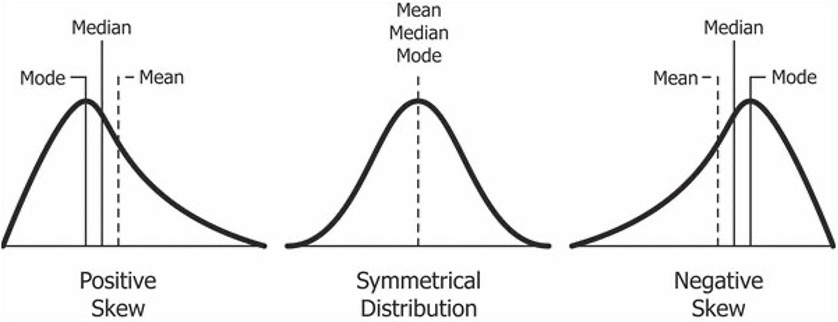
\includegraphics[scale=0.4]{test-2/mean-median-mode}
     \end{figure}
     \item Examples:
     \begin{enumerate}\setcounter{enumi}{3}
        \item Find the IQR of $X$ using the following cdf:
        \item[] $\displaystyle F(x) = P(X \le x) = 1 - \frac{1}{x^2}, \quad\quad 1 \le x < \infty$.\vspace{130pt}
        \item The time $X$ in months until failure of a certain product has the pdf 
        \item[] $f(x) = (1/2)\,x\,\e^{-(x/2)^2} \quad \text{for } 0 < x < \infty$.
        \item[] Find the first and second quartiles of $X$.\vspace{150pt}

     \end{enumerate}
\end{itemize}\bigskip




\end{document}